\begin{question}
\noindent Triangle $T$ has vertices $A(1,2)$, $B(1,4)$ and $C(3,2)$.

The point $P(-1,1)$ is marked as the centre of rotation.

\begin{center}
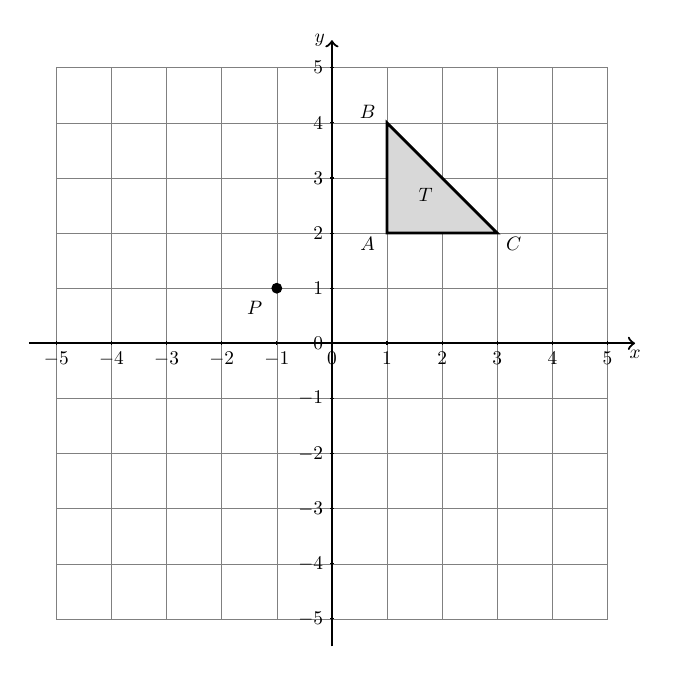
\begin{tikzpicture}[scale=0.7, transform shape]
    \def\axisLimit{5}

    \definecolor{borderColour}{HTML}{000000}
    \definecolor{fillColour}{HTML}{D8D8D8}

    % Draw grid
    \draw[step=1cm,gray,very thin] (-\axisLimit,-\axisLimit) grid (\axisLimit,\axisLimit);

    % Draw axes
    \draw[thick,->] (-\axisLimit-0.5,0) -- (\axisLimit+0.5,0) node[anchor=north] {$x$};
    \draw[thick,->] (0,-\axisLimit-0.5) -- (0,\axisLimit+0.5) node[anchor=east] {$y$};

    % Label x-axis and y-axis
    \foreach \x in {-\axisLimit,...,\axisLimit}
        \draw (\x cm,1pt) -- (\x cm,-1pt) node[anchor=north] {$\x$};
    \foreach \y in {-\axisLimit,...,\axisLimit}
        \draw (1pt,\y cm) -- (-1pt,\y cm) node[anchor=east] {$\y$};

    % Define coordinates for triangle T
    \coordinate (A) at (1,2);
    \coordinate (B) at (1,4);
    \coordinate (C) at (3,2);

    % Draw triangle T
    \filldraw[fill=fillColour, draw=borderColour, line width=1pt] (A) -- (B) -- (C) -- cycle;
    \node at (0.65,1.8) {$A$};
    \node at (0.65,4.2) {$B$};
    \node at (3.3,1.8) {$C$};
    \node at (1.7,2.7) {$T$};

    % Mark the centre of rotation P
    \coordinate (P) at (-1,1);
    \filldraw[black] (P) circle (2.5pt);
    \node at (-1.4,0.65) {$P$};

\end{tikzpicture}
\end{center}

\noindent On the grid, draw the image of triangle $T$ after a rotation of $90^\circ$ clockwise about the point $P$.

\vspace{4cm}
\answermarks{3}
\end{question}
